% Adjust these for the path of the theme and its graphics, relative to this file
%\usepackage{beamerthemeFalmouthGamesAcademy}
\usepackage{../../beamerthemeFalmouthGamesAcademy}
\graphicspath{ {../../} }

% Default language for code listings
\lstset{language=[Sharp]C
}

% For strikethrough effect
\usepackage[normalem]{ulem}
\usepackage{wasysym}

\usepackage{pdfpages}

\usepackage{algpseudocode}
\usepackage{qtree}

% http://www.texample.net/tikz/examples/state-machine/
\usetikzlibrary{arrows,automata}
\usetikzlibrary{tikzmark,calc}

\newcommand{\modulecode}{COMP260}\newcommand{\moduletitle}{Distributed Systems}\newcommand{\sessionnumber}{5}

\begin{document}
\title{\sessionnumber: Algorithm Strategies}
\subtitle{\modulecode: \moduletitle}

\frame{\titlepage} 

\begin{frame}{Worksheets}
	\begin{itemize}
		\item Worksheet 6: due \textbf{this Wedensday}
		\item Worksheet 7: due \textbf{next Wedensday}
	\end{itemize}
\end{frame}

\part{Recursion}
\frame{\partpage}

\begin{frame}[fragile]{Recursion}
    \begin{itemize}
        \pause\item A \textbf{recursive} function is a function that \textbf{calls itself}
    \end{itemize}
    \pause
    \begin{lstlisting}
int factorial(int n)
{
    if (n <= 1)
        return 1;
    else
        return n * factorial(n-1);
}
    \end{lstlisting}
    \begin{itemize}
        \pause\item Recursive functions need a \textbf{base case} where they stop recursing,
			otherwise they will go \textbf{forever}
        \pause\item (Or rather, until a \textbf{stack overflow})
    \end{itemize}
\end{frame}

\begin{frame}{Thinking recursively}
	\begin{itemize}
		\pause\item I want to solve a problem
		\pause\item If I already had a function to solve smaller instances of the problem, I could use it
			to write my function
		\pause\item I can solve the smallest possible problem
		\pause\item Therefore I can write a recursive function
	\end{itemize}
\end{frame}

\begin{frame}{The call stack}
	\begin{itemize}
		\pause\item Recall: nested function calls are handled using a \textbf{stack}
		\pause\item Recursive functions are no different
		\pause\item This means if a recursive function contains \textbf{local variables},
			they are \textbf{independent} between instances of the function
	\end{itemize}
\end{frame}

\part{Graphs and trees}
\frame{\partpage}

\begin{frame}{Graphs}
	\begin{columns}
		\pause
		\begin{column}{0.3\textwidth}
			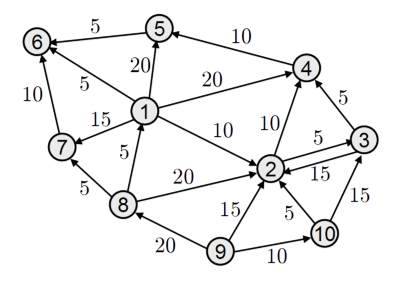
\includegraphics[width=\textwidth]{graph1}
			\par
			\vspace{2ex}
			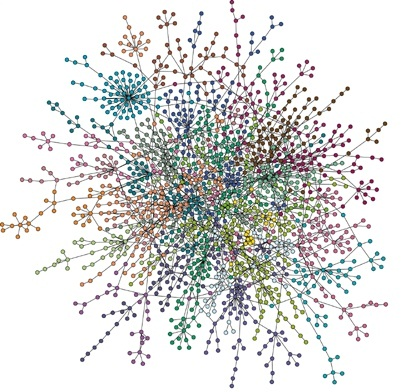
\includegraphics[width=\textwidth]{graph2}
		\end{column}
		\begin{column}{0.68\textwidth}
			\begin{itemize}
				\pause\item A \textbf{graph} is defined by:
					\begin{itemize}
						\pause\item A collection of \textbf{nodes} or \textbf{vertices} (points)
						\pause\item A collection of \textbf{edges} or \textbf{arcs} (lines or arrows between points)
					\end{itemize}
				\pause\item Often used to model \textbf{networks} (e.g.\ social networks, transport networks, game levels, automata, ...)
				\pause\item \textbf{Directed} graph: edges are arrows
				\pause\item \textbf{Undirected} graph: edges are lines
			\end{itemize}
		\end{column}
	\end{columns}
\end{frame}

\begin{frame}{Drawing graphs}
    \begin{itemize}
        \pause\item A graph does not necessarily specify the physical \textbf{positions} of its nodes
        \pause\item E.g.\ these are technically the same graph:
    \end{itemize}
    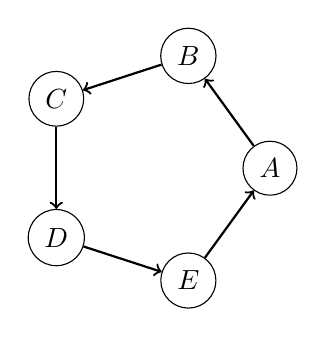
\begin{tikzpicture}
        \node[draw, circle] (a) at (0:1.5) {$A$};
        \node[draw, circle] (b) at (72:1.5) {$B$};
        \node[draw, circle] (c) at (144:1.5) {$C$};
        \node[draw, circle] (d) at (216:1.5) {$D$};
        \node[draw, circle] (e) at (288:1.5) {$E$};
        \draw[thick,->] (a) -- (b);
        \draw[thick,->] (b) -- (c);
        \draw[thick,->] (c) -- (d);
        \draw[thick,->] (d) -- (e);
        \draw[thick,->] (e) -- (a);
    \end{tikzpicture}
    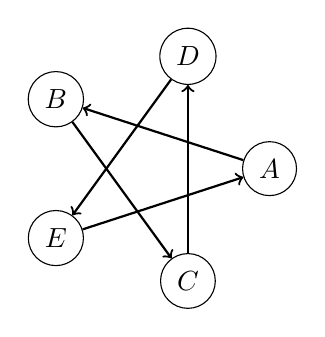
\begin{tikzpicture}
        \node[draw, circle] (a) at (0:1.5) {$A$};
        \node[draw, circle] (b) at (144:1.5) {$B$};
        \node[draw, circle] (c) at (288:1.5) {$C$};
        \node[draw, circle] (d) at (72:1.5) {$D$};
        \node[draw, circle] (e) at (216:1.5) {$E$};
        \draw[thick,->] (a) -- (b);
        \draw[thick,->] (b) -- (c);
        \draw[thick,->] (c) -- (d);
        \draw[thick,->] (d) -- (e);
        \draw[thick,->] (e) -- (a);
    \end{tikzpicture}
    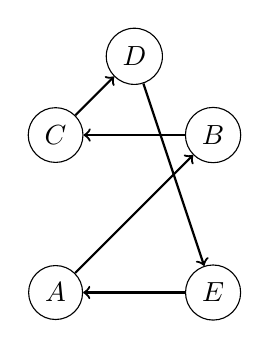
\begin{tikzpicture}
        \node[draw, circle] (a) at (0,0) {$A$};
        \node[draw, circle] (b) at (2,2) {$B$};
        \node[draw, circle] (c) at (0,2) {$C$};
        \node[draw, circle] (d) at (1,3) {$D$};
        \node[draw, circle] (e) at (2,0) {$E$};
        \draw[thick,->] (a) -- (b);
        \draw[thick,->] (b) -- (c);
        \draw[thick,->] (c) -- (d);
        \draw[thick,->] (d) -- (e);
        \draw[thick,->] (e) -- (a);
    \end{tikzpicture}
\end{frame}

\begin{frame}{Trees}
	\begin{columns}
		\pause
		\begin{column}{0.3\textwidth}
			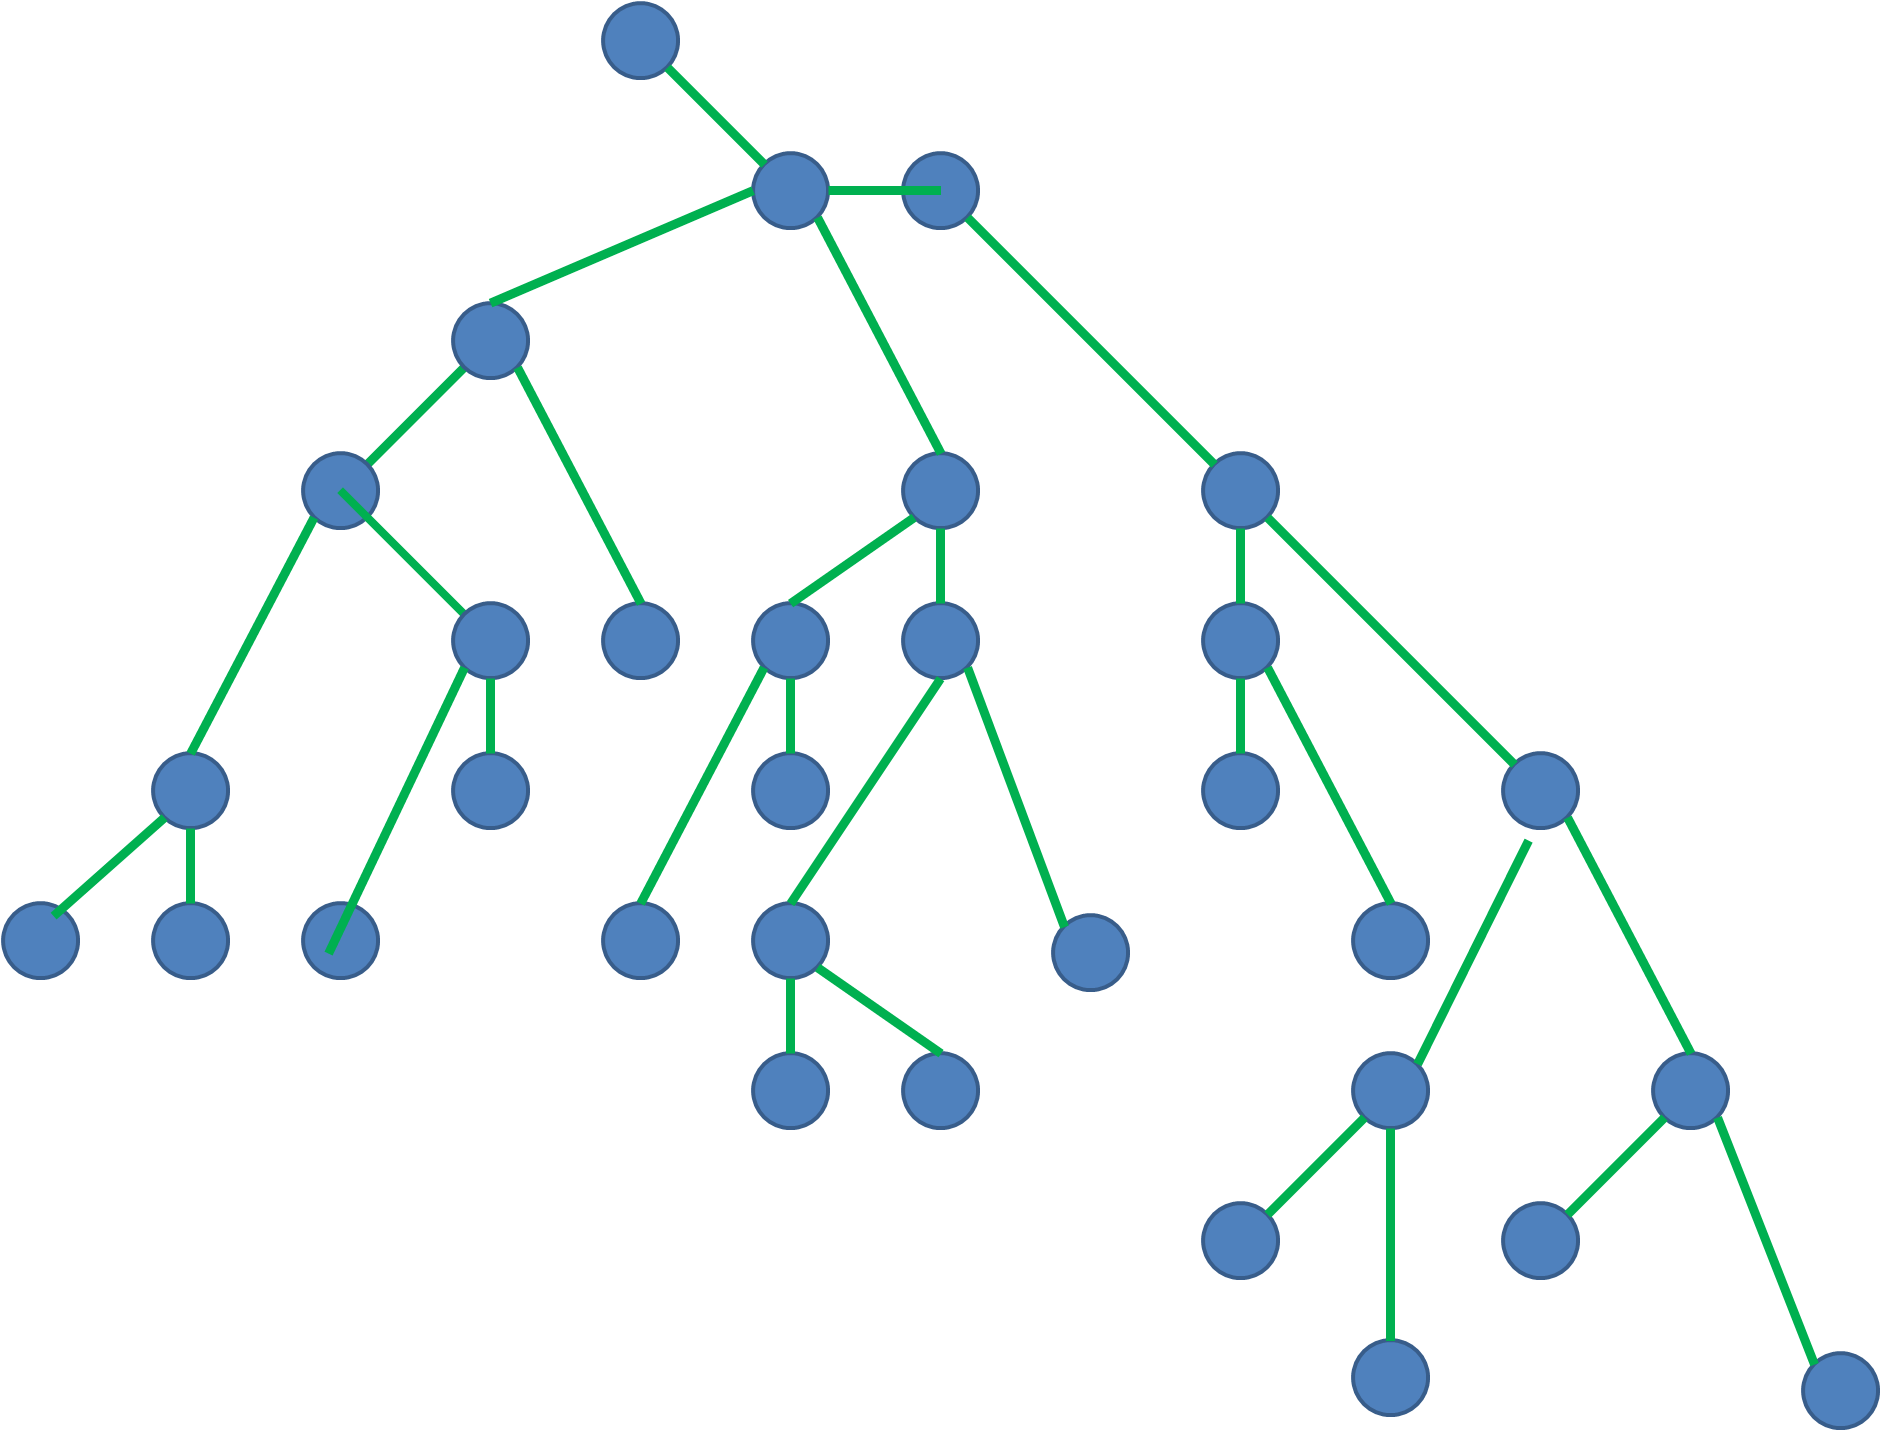
\includegraphics[width=\textwidth]{tree2}
			\par
			\vspace{2ex}
			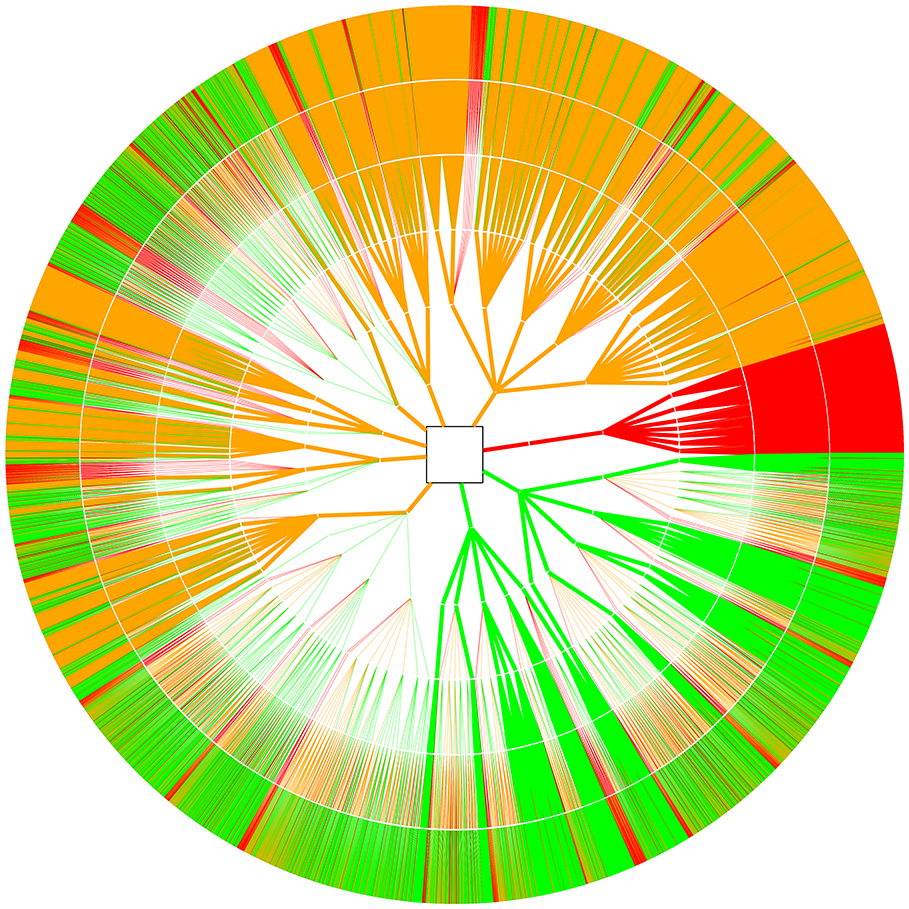
\includegraphics[width=\textwidth]{tree}
		\end{column}
		\begin{column}{0.68\textwidth}
			\begin{itemize}
				\pause\item A \textbf{tree} is a special type of directed graph where:
					\begin{itemize}
						\pause\item One node (the \textbf{root}) has no incoming edges
						\pause\item All other nodes have exactly 1 incoming edge
					\end{itemize}
				\pause\item Edges go from \textbf{parent} to \textbf{child}
					\begin{itemize}
						\pause\item All nodes except the root have exactly one parent
						\pause\item Nodes can have 0, 1 or many children
					\end{itemize}
				\pause\item Used to model \textbf{hierarchies} (e.g.\ file systems, object inheritance, scene graphs, state-action trees, behaviour trees, ...)
			\end{itemize}
		\end{column}
	\end{columns}
\end{frame}

\part{Tree traversal}
\frame{\partpage}

\begin{frame}{Tree traversal}
	\begin{itemize}
		\pause\item \textbf{Traversal}: visiting all the nodes of the tree
		\pause\item Two main types
			\begin{itemize}
				\pause\item Depth first
				\pause\item Breadth first
			\end{itemize}
	\end{itemize}
\end{frame}

\begin{frame}{Tree traversal}
	\pause\footnotesize
%	\begin{columns}
%		\begin{column}{0.48\textwidth}
			\begin{algorithmic}
				\Procedure{DepthFirstSearch}{} \pause
					\State let $S$ be a stack \pause
					\State push root node onto $S$ \pause
					\While{$S$ is not empty} \pause
						\State pop $n$ from $S$ \pause
						\State print $n$ \pause
						\State push children of $n$ onto $S$ \pause
					\EndWhile
				\EndProcedure
			\end{algorithmic}
%		\end{column}
		\pause
%		\begin{column}{0.48\textwidth}
		\vspace{2ex}
			\begin{algorithmic}
				\Procedure{BreadthFirstSearch}{} \pause
					\State let $Q$ be a queue \pause
					\State enqueue root node into $Q$ \pause
					\While{$Q$ is not empty} \pause 
						\State dequeue $n$ from $Q$ \pause
						\State print $n$ \pause
						\State enqueue children of $n$ into $Q$ \pause
					\EndWhile
				\EndProcedure
			\end{algorithmic}
%		\end{column}
%	\end{columns}
\end{frame}

\begin{frame}{Tree traversal example}
	\begin{center}
		Socrative \texttt{FALCOMPED}
	\end{center}
	\Tree
		[.A
			[.Z
				[.N
				]
				[.S
					[.Q
						[.R
						]
						[.P
						]
					]
					[.W
						[.E
						]
						[.G
						]
						[.X
						]
					]
				]
				[.B
					[.L
						[.M
						]
						[.U
						]
					]
					[.I
					]
				]
			]
			[.K
				[.H
				]
				[.Y
					[.V
						[.T
						]
					]
					[.C
					]
				]
				[.D
				]
			]
		]
\end{frame}


\begin{frame}{Recursive depth first search}
	\pause
	\begin{algorithmic}
		\Procedure{DepthFirstSearch}{$n$} \pause
			\State print $n$ \pause
			\For{\textbf{each} child $c$ of $n$} \pause
				\State \Call{DepthFirstSearch}{$c$} \pause
			\EndFor
		\EndProcedure
	\end{algorithmic}
	\begin{itemize}
		\pause\item Compare to the pseudocode on the previous slide. Where is the stack?
	\end{itemize}
\end{frame}


\part{Algorithm strategies}
\frame{\partpage}

\newcommand{\weight}{\operatorname{weight}}
\newcommand{\val}{\operatorname{value}}
\newcommand{\best}{{\text{best}}}

\begin{frame}{The knapsack problem}
	\begin{itemize}
		\pause\item There is a set $X$ of \textbf{items}
		\pause\item Each item $x$ has a weight $\weight(x)$ and a value $\val(x)$
		\pause\item There is a maximum weight $W$
		\pause\item What subset $S \subseteq X$ maximises the total value, whilst not exceeding the maximum weight?
		\pause\item In other words: find $S \subseteq X$ to maximise
			$$ \sum_{x \in S} \val(x) $$
		subject to
			$$ \sum_{x \in S} \weight(x) \leq W $$
	\end{itemize}
\end{frame}

\begin{frame}{Algorithm strategies}
	\begin{itemize}
		\pause\item Brute force
		\pause\item Greedy
		\pause\item Divide-and-conquer
		\pause\item Dynamic programming
	\end{itemize}
\end{frame}

\begin{frame}{Brute force}
	\begin{itemize}
		\pause\item Try \textbf{every possible} solution and decide which is best
	\end{itemize}
	\pause
	\begin{algorithmic}
		\Procedure{Knapsack}{X, W}
			\pause\State $S_\best \gets \{ \}$
			\pause\State $v_\best \gets 0$
			\pause\For{every subset $S \subseteq X$}
				\pause\If{$\weight(S) \leq W$ and $\val(S) > v_\best$}
					\pause\State $S_\best \gets S$
					\pause\State $v_\best \gets \val(S)$
				\pause\EndIf
			\pause\EndFor
			\pause\State \textbf{return} $S_\best$
		\pause\EndProcedure
	\end{algorithmic}
\end{frame}

\begin{frame}{Socrative \texttt{FALCOMPED}}
	\begin{itemize}
		\pause\item If $X$ contains $n$ elements, how many subsets of $X$ are there?
		\pause\item Therefore what is the time complexity of the brute force algorithm?
		\pause\item If we add one element to $X$, what happens to the running time of the algorithm?
	\end{itemize}
\end{frame}

\begin{frame}{Greedy algorithm}
	\begin{itemize}
		\pause\item At each stage of building a solution, take the \textbf{best} available option
	\end{itemize}
	\pause
	\begin{algorithmic}
		\Procedure{Knapsack}{X, W}
			\pause\State $S \gets \{ \}$
			\pause\For{each $x \in X$, in descending order of $\val(x)$}
				\pause\If{$\weight(S) + \weight(x) \leq W$}
					\pause\State add $x$ to $S$
				\pause\EndIf
			\pause\EndFor
			\pause\State \textbf{return} $S$
		\EndProcedure
	\end{algorithmic}
\end{frame}

\begin{frame}{Greedy algorithm}
	\begin{itemize}
		\pause\item Time complexity is dominated by sorting $X$ by value
		\pause\item The rest of the algorithm runs in linear time
		\pause\item In some problems an appropriately chosen greedy solution is \textbf{optimal}
			\begin{itemize}
				\pause\item A$^*$ pathfinding
				\pause\item Huffman coding
			\end{itemize}
		\pause\item \textbf{However} the greedy solution to the knapsack problem may not be optimal!
	\end{itemize}
\end{frame}

\begin{frame}{Divide and conquer}
	\begin{itemize}
		\pause\item Break the problem into smaller, easier to solve \textbf{subproblems}
		\pause\item Requires that the solution to the original problem is composed of the solutions to the smaller problem
		\pause\item Example from last time: \textbf{binary search}
			\begin{itemize}
				\pause\item Problem: find an element in a list
				\pause\item Subproblem: find the element in a list of half the size
			\end{itemize}
	\end{itemize}
\end{frame}

\begin{frame}{Divide and conquer for the knapsack problem}
	\begin{itemize}
		\pause\item Consider an element $x \in X$ with $\weight(x) \leq W$
		\pause\item Let $X'$ be $X$ with $x$ removed
		\pause\item The solution to the knapsack problem either includes $x$ or it doesn't
		\pause\item The solution is \textbf{either}:
			\begin{itemize}
				\pause\item The solution to the knapsack problem on $X'$ with maximum weight $W$, \textbf{or}
				\pause\item The solution to the knapsack problem on $X'$ with maximum weight $W - \weight(x)$,
					plus $x$
			\end{itemize}
		\pause\item ... whichever has the greater value
		\pause\item Base case: the solution to the knapsack problem on the empty set \textbf{is} the empty set
	\end{itemize}
\end{frame}

\begin{frame}{Divide and conquer for the knapsack problem}
	\begin{algorithmic}
		\pause\Procedure{Knapsack}{X, W, k}
			\pause\If{$k < 0$}
				\pause\State \textbf{return} $\{\}$
			\pause\EndIf
			
			\pause\State $S \gets \Call{Knapsack}{X, W, k-1}$
			\pause\If{$\weight(x_k) \leq W$}
				\pause\State $S' \gets \Call{Knapsack}{X, W - \weight(x_k), k-1} \cup \{x_k\}$
				\pause\State \textbf{return} whichever of $S,S'$ has the larger value
			\pause\Else
				\pause\State \textbf{return} $S$
			\pause\EndIf
		\pause\EndProcedure
	\end{algorithmic}
\end{frame}

\begin{frame}{Time complexity}
	\begin{itemize}
		\pause\item Each call to \Call{Knapsack}{} has, in the worst case, \textbf{two} recursive calls to \Call{Knapsack}{}
		\pause\item Number of calls is
			$$ \underbrace{1 + 2 + 4 + 8 + \dots + 2^i + \dots}_{\text{$n$ terms}} $$
		\pause\item Thus the worst case time complexity is $O(2^n)$ --- still exponential!
		\pause\item However in the \textbf{average} case many of the calls have only a single recursive call,
			so this is still more efficient than brute force
	\end{itemize}
\end{frame}

\begin{frame}{Overlapping subproblems}
	\begin{itemize}
		\pause\item Here we end up solving the \textbf{same subproblem multiple times}
		\pause\item Can save time by \textbf{caching} (remembering) these sub-solutions
		\pause\item This is called \textbf{memoization}
		\pause\item One of several techniques in the category of \textbf{dynamic programming}
	\end{itemize}
\end{frame}

\begin{frame}{Dynamic programming for the knapsack problem}
	\begin{algorithmic}
		\pause\Procedure{Knapsack}{X, W, k}
			\pause\If{\Call{Knapsack}{X, W, k} has already been computed}
				\pause\State \textbf{return} previously computed result
			\pause\EndIf
			
			\pause\If{$k < 0$}
				\State \textbf{cache and return} $\{\}$
			\EndIf
			
			\State $S \gets \Call{Knapsack}{X, W, k-1}$
			\If{$\weight(x_k) \leq W$}
				\State $S' \gets \Call{Knapsack}{X, W - \weight(x_k), k-1} \cup \{x_k\}$
				\State \textbf{cache and return} whichever of $S,S'$ has the larger value
			\Else
				\State \textbf{cache and return} $S$
			\EndIf
		\EndProcedure
	\end{algorithmic}
\end{frame}

\begin{frame}{Socrative \texttt{FALCOMPED}}
	\begin{itemize}
		\pause\item What is the maximum possible number of entries in the table of intermediate results?
		\pause\item Therefore what is the time complexity of the dynamic programming algorithm?
	\end{itemize}
\end{frame}

\begin{frame}{Summary of algorithm strategies}
	\begin{itemize}
		\pause\item Brute force
			\begin{itemize}
				\pause\item Good enough for small/simple problems
			\end{itemize}
		\pause\item Greedy
			\begin{itemize}
				\pause\item Efficient for certain problems, but doesn't always give optimal solutions
			\end{itemize}
		\pause\item Divide-and-conquer
			\begin{itemize}
				\pause\item Good if the problem can be broken down into simpler subproblems
			\end{itemize}
		\pause\item Dynamic programming
			\begin{itemize}
				\pause\item Makes divide-and-conquer more efficient if subproblems often reoccur
			\end{itemize}
	\end{itemize}
\end{frame}



\part{Workshop}
\frame{\partpage}

\end{document}
